\section{Ergebnisse} % (fold)
    \label{sec:ergebnisse}
    Die der Durchführung der Experimente läuft nach einem immergleichen Schema ab. Zuerst werden mit den MapMan-Proteinen aus \autoref{sub:mapman} die Datenbanken erstellt und anschließend mit einer Teilmenge dieser Proteine das Matching durchgeführt. Zumindest mit den \aclp{TP} als Eingabe sollten bei korrekten Parametern erwartbar gute Ergebnisse erzielt werden, sodass hier Konzeptfehler sehr schnell auffallen. Neben den experimentspezifischen Parametern, wie Quantilen oder der Größe der \acl{TZ}, werden zusätzlich jedes Mal Parameter getestet, die die \ac{STFT} betreffen, da sich diese aufgrund der zu digitaler Musik vergleichsweise kurzen Sequenzen nicht direkt von SHAZAM ableiten lassen. Solche Parameter sind hier die Fenstergröße, welche in 10er-Schritten von 10\-50 betrachtet werden, die Überlappung zwischen benachbarten Fenstern, hier 25, 50 und 75 Prozent der Fenstergröße, und $n\_peaks$, der Anzahl Frequenzen, die von der Selektion verwendet werden, welche unabhängig von $k$ aus \hyperref[exp:selection_method]{Experiment 4} ist.

    Die Wahl der Proteine für das Matching geschieht folgendermaßen:

    \subsection{UniRef90 Sampling} % (fold)
        \label{sub:uniref90_results}
        \begin{figure}[H]
            \centering
            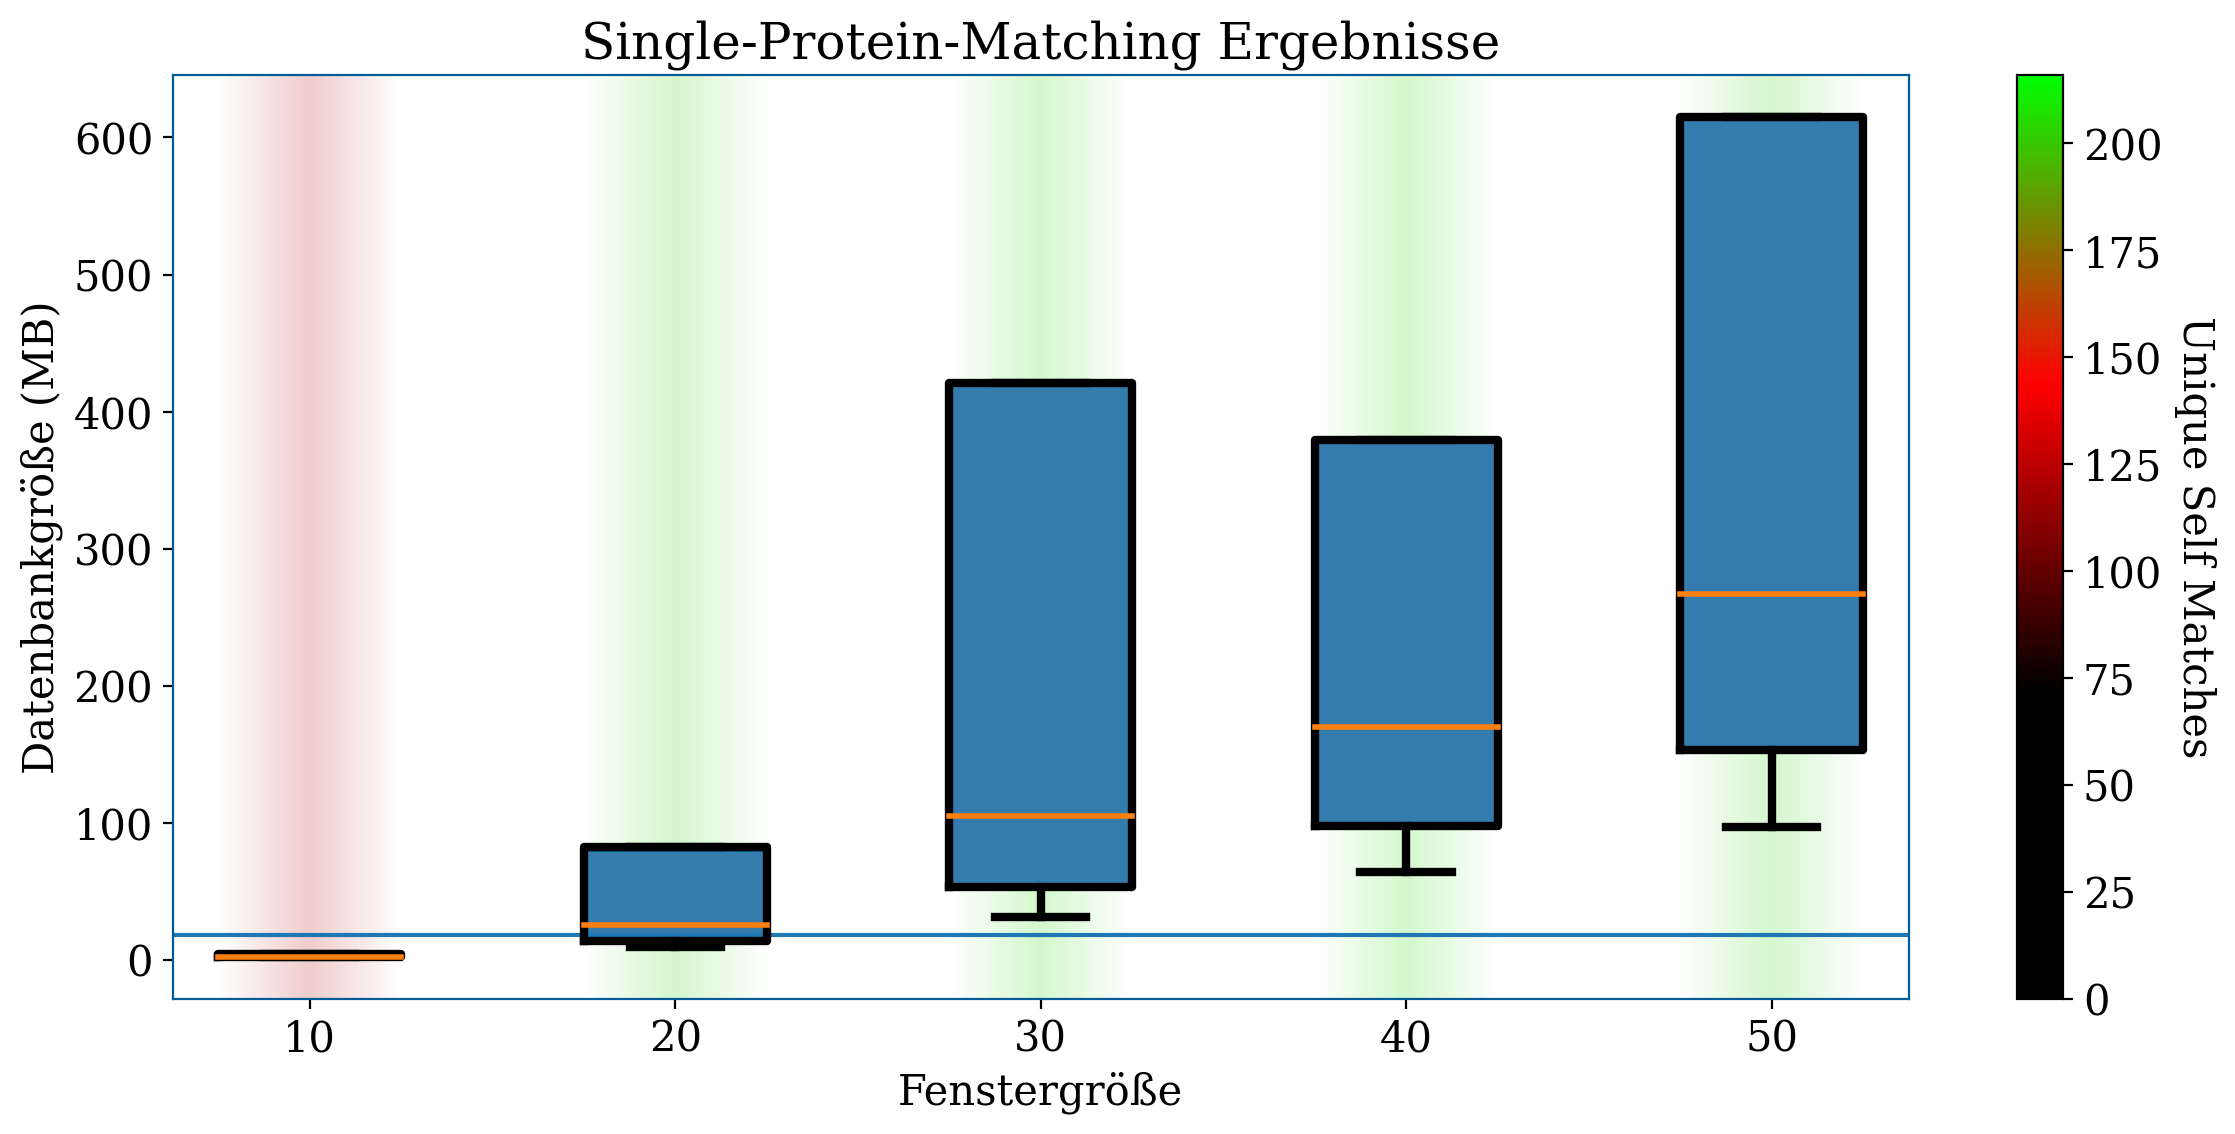
\includegraphics[width=\textwidth]{plot_uniref90.sp.png}
            \caption{bla}
            \label{fig:uniref90.sp}
        \end{figure}
        \begin{figure}[H]
            \centering
            \begin{subfigure}{.45\textwidth}
                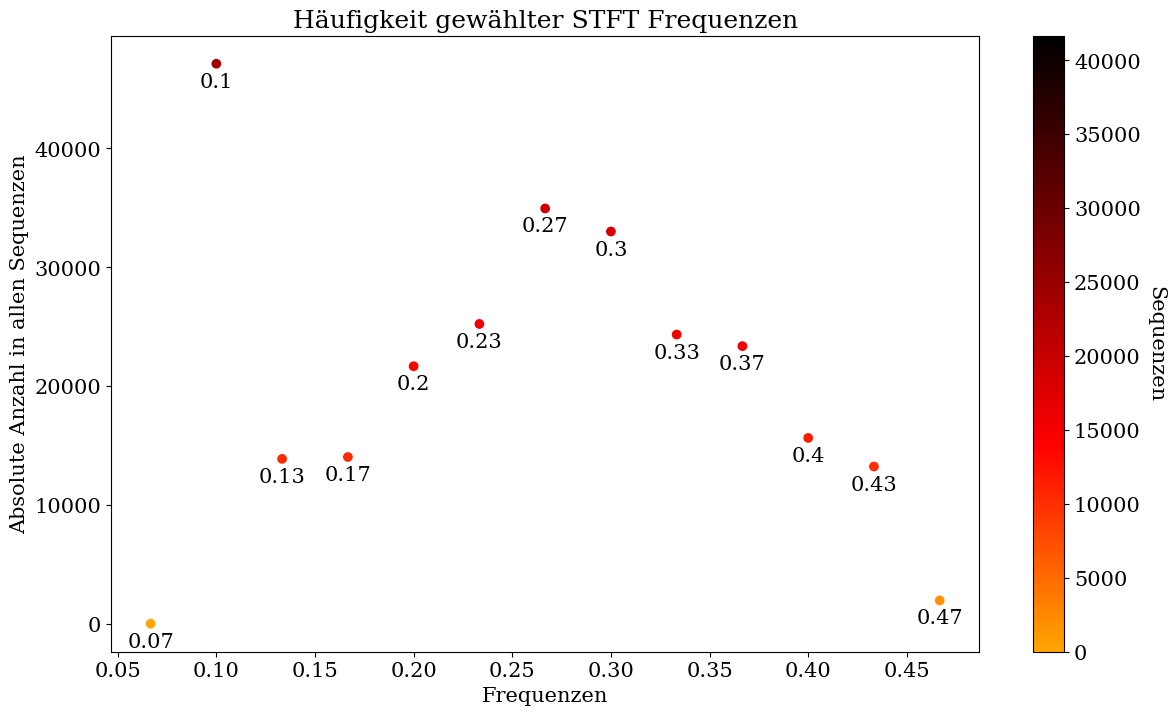
\includegraphics[width=\textwidth]{frequencies_5.png}
                \caption{$\alpha=5\%$}
                \label{fig:frequencies_5}
            \end{subfigure}
            \begin{subfigure}{.45\textwidth}
                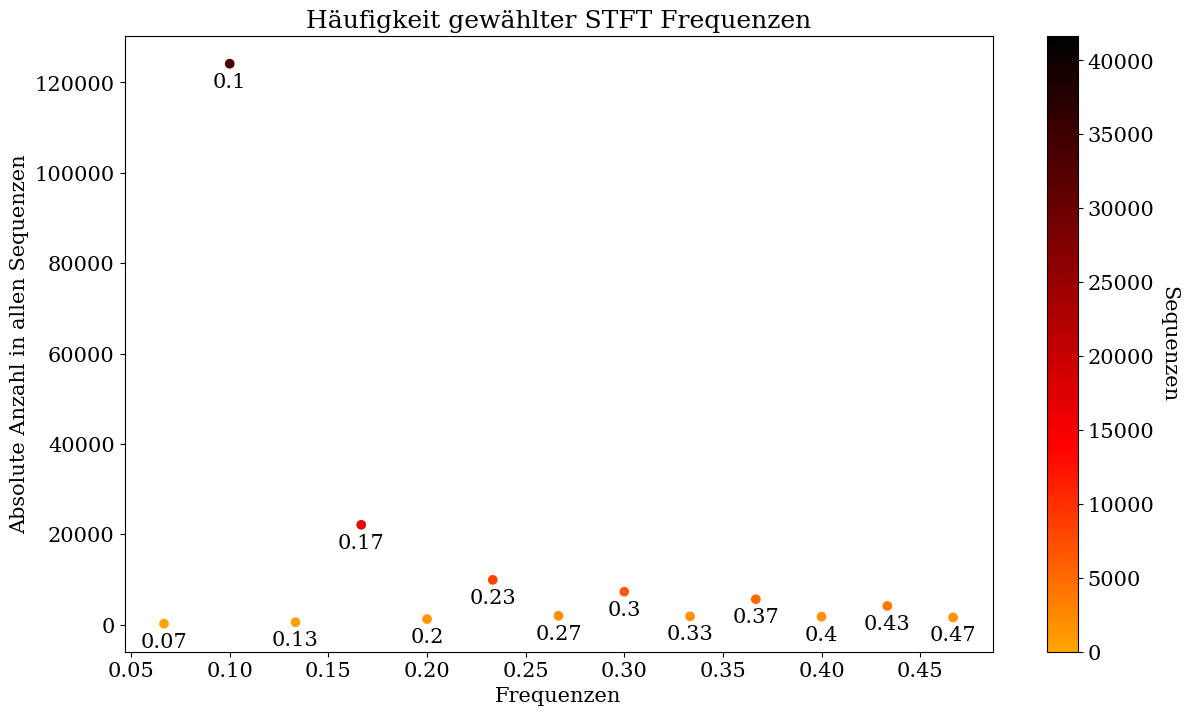
\includegraphics[width=\textwidth]{frequencies_0.1.png}
                \caption{$\alpha=0.1\%$}
                \label{fig:frequencies_0.1}
            \end{subfigure}\\
            \begin{subfigure}{.45\textwidth}
                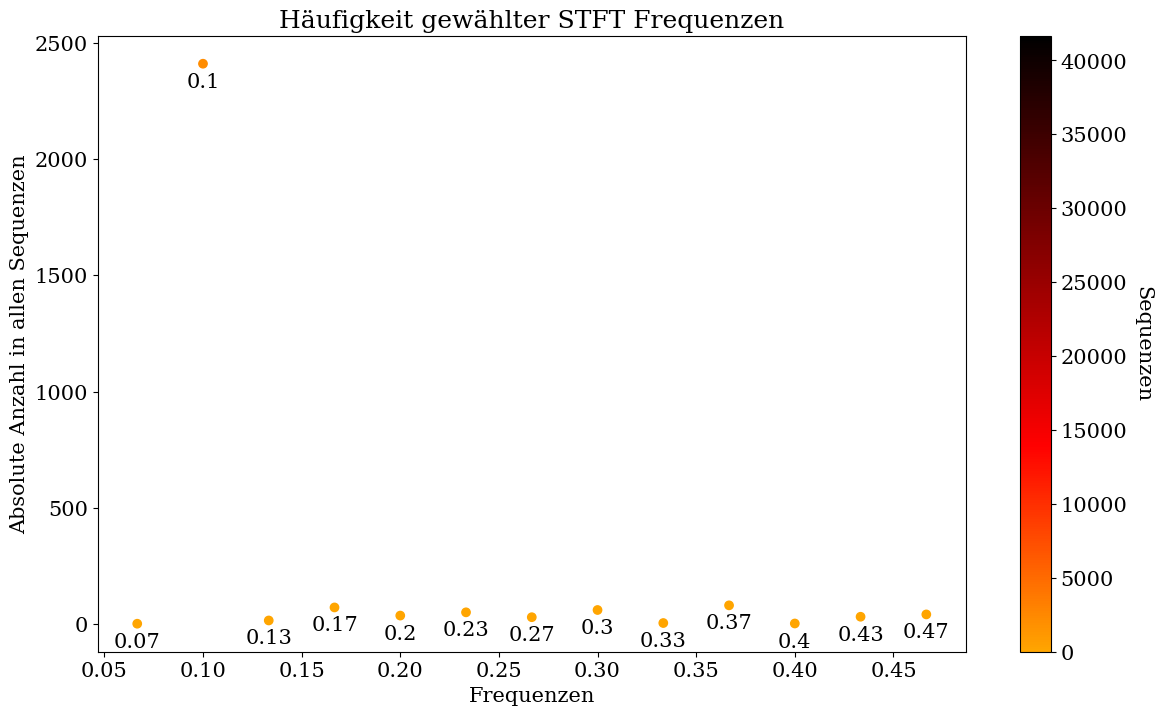
\includegraphics[width=\textwidth]{frequencies_0.01.png}
                \caption{$\alpha=0.01\%$}
                \label{fig:frequencies_0.01}
            \end{subfigure}
            \begin{subfigure}{.45\textwidth}
                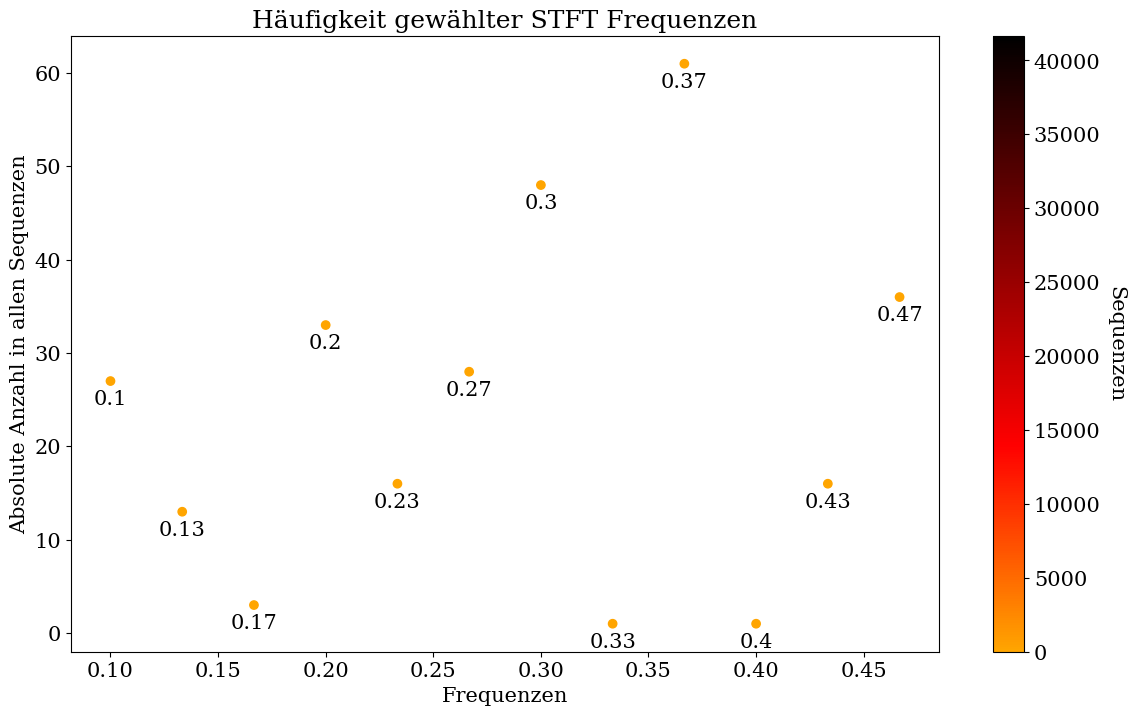
\includegraphics[width=\textwidth]{frequencies_0.001.png}
                \caption{$\alpha=0.001\%$}
                \label{fig:frequencies_0.001}
            \end{subfigure}\\
            \begin{subfigure}{.45\textwidth}
                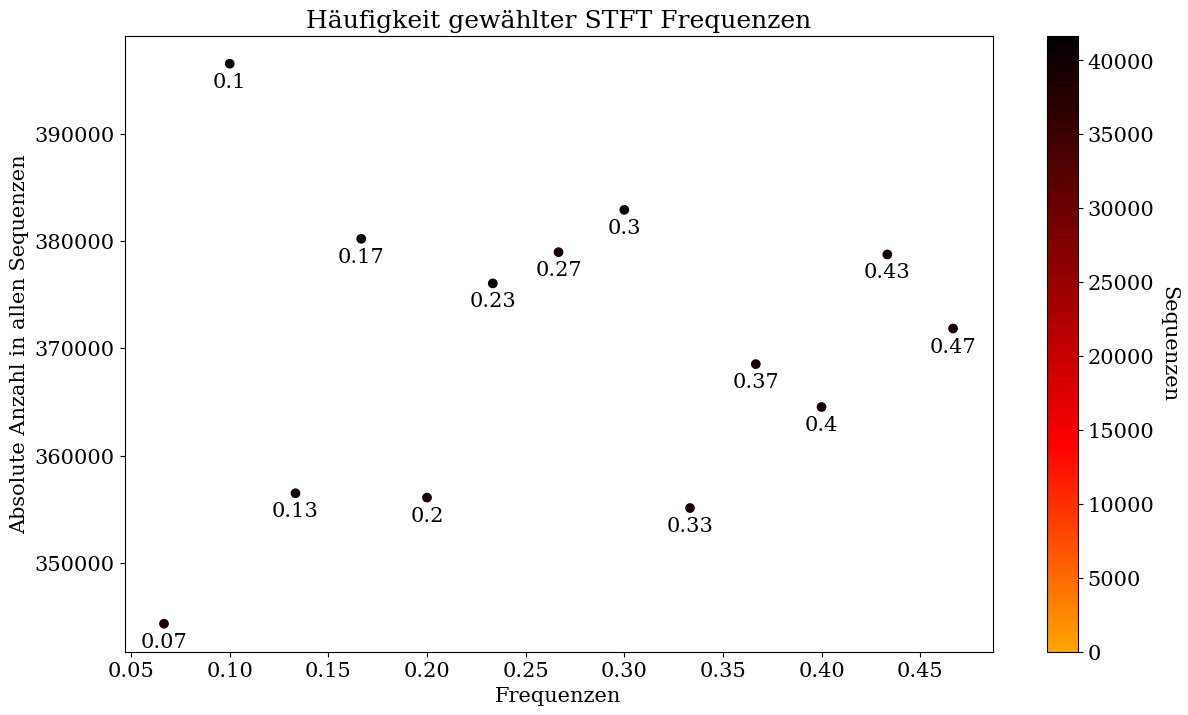
\includegraphics[width=\textwidth]{frequencies_normal.png}
                \caption{Normal}
                \label{fig:frequencies_normal}
            \end{subfigure}
            \caption{Häufigkeit gewählter Frequenzen über alle \aclp{TP}}
            \label{fig:frequencies}
        \end{figure}
    
    % subsection uniref90_sampling (end)
    \subsection{Filter Hashes} % (fold)
        \label{sub:filter_results}
        \begin{figure}[H]
            \centering
            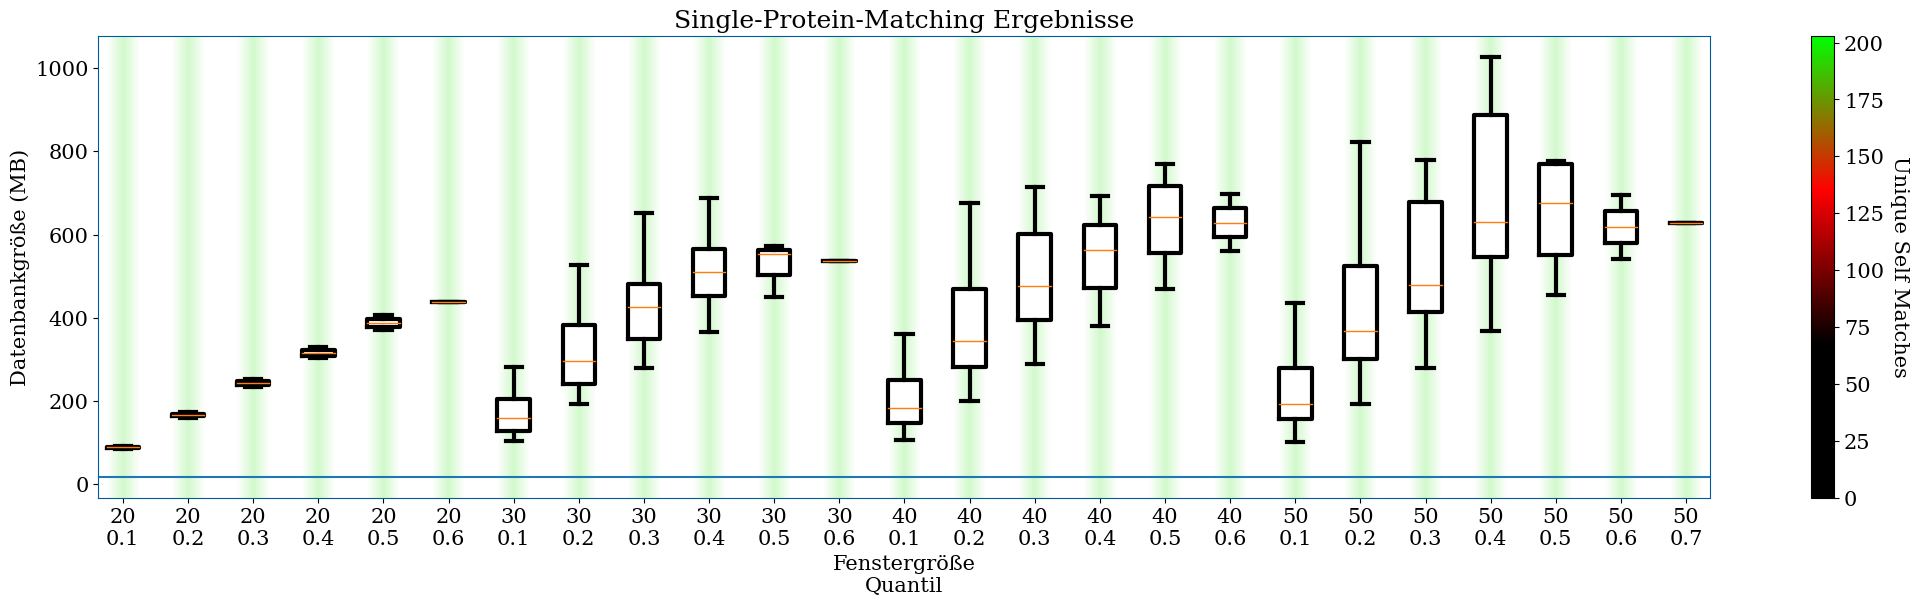
\includegraphics[width=\textwidth]{plot_filter_hashes.sp.png}
            \caption{bla}
            \label{fig:filter_hashes.sp}
        \end{figure}
        \begin{figure}[H]
            \centering
            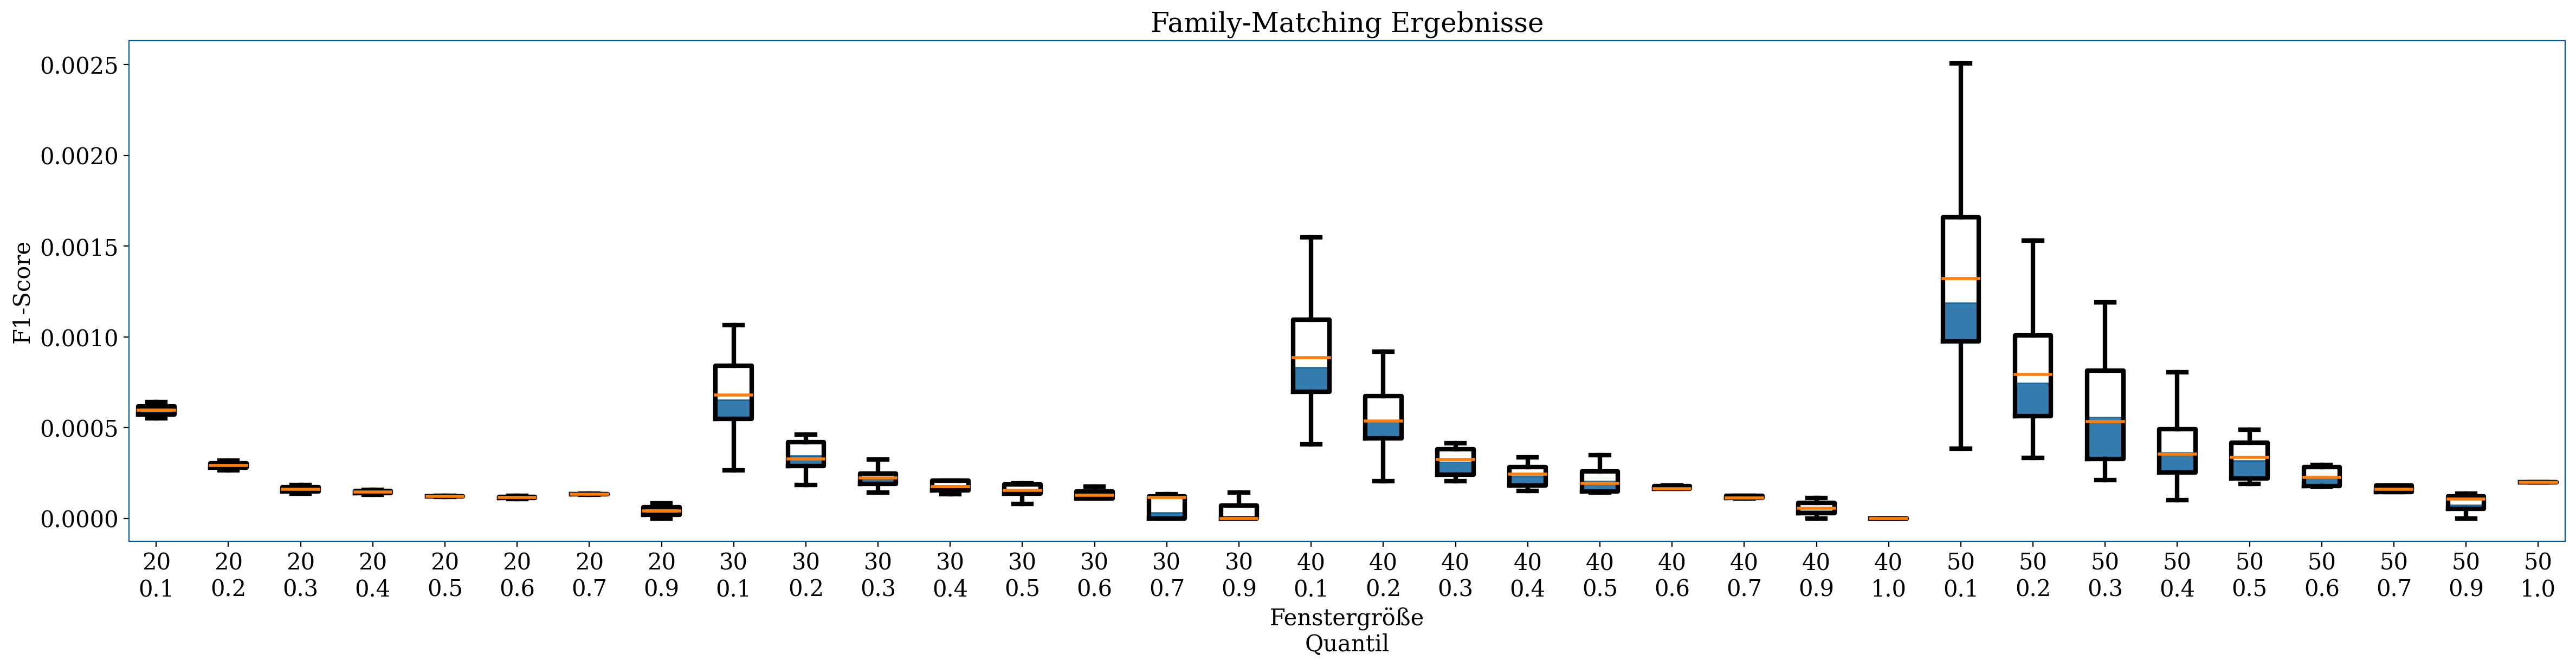
\includegraphics[width=\textwidth]{plot_filter_hashes.fam.png}
            \caption{bla}
            \label{fig:filter_hashes.fam}
        \end{figure}

    \subsection{Target-Zone} % (fold)
        \label{sub:target_results}
        \begin{figure}[H]
            \centering
            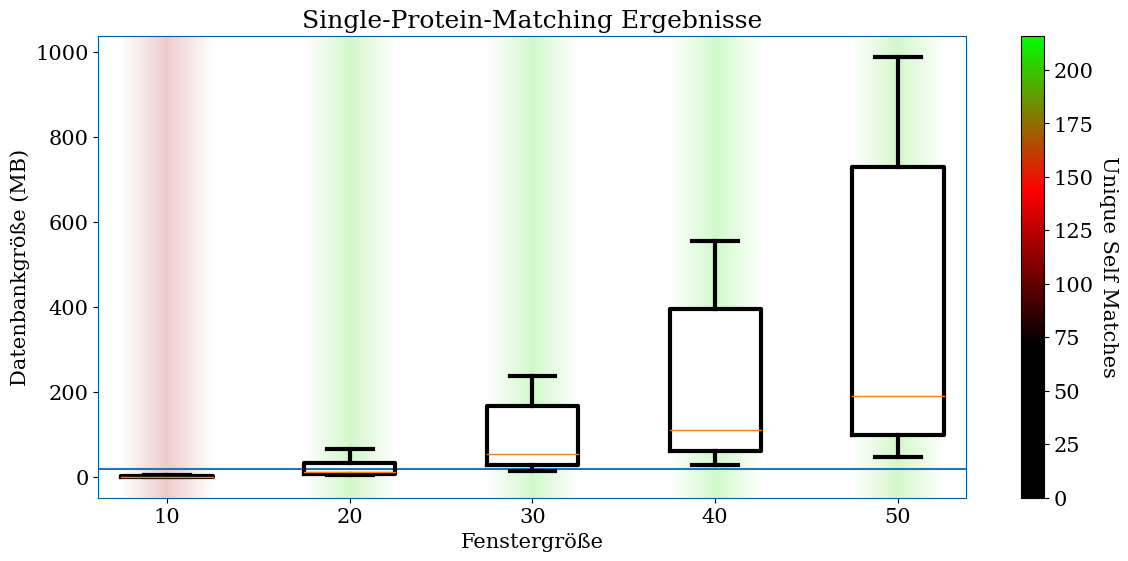
\includegraphics[width=\textwidth]{plot_target_zone.sp.png}
            \caption{bla}
            \label{fig:target_zone.sp}
        \end{figure}

    \subsection{Selection-Method} % (fold)
        \label{sub:selection_results}
        \begin{figure}[H]
            \centering
            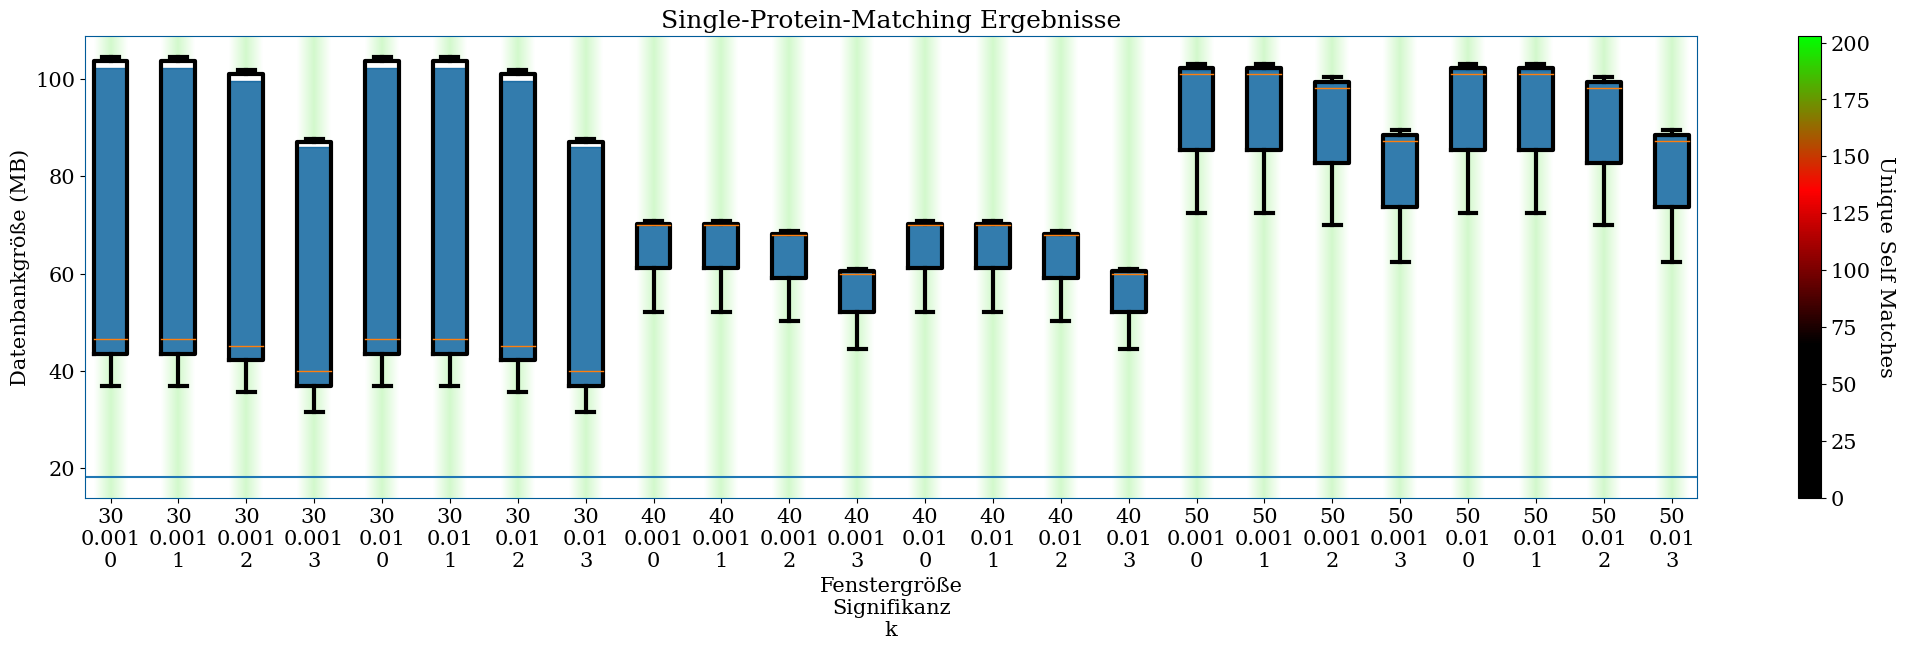
\includegraphics[width=\textwidth]{plot_selection_method.sp.png}
            \caption{bla}
            \label{fig:selection_method.sp}
        \end{figure}
        \begin{figure}[H]
            \centering
            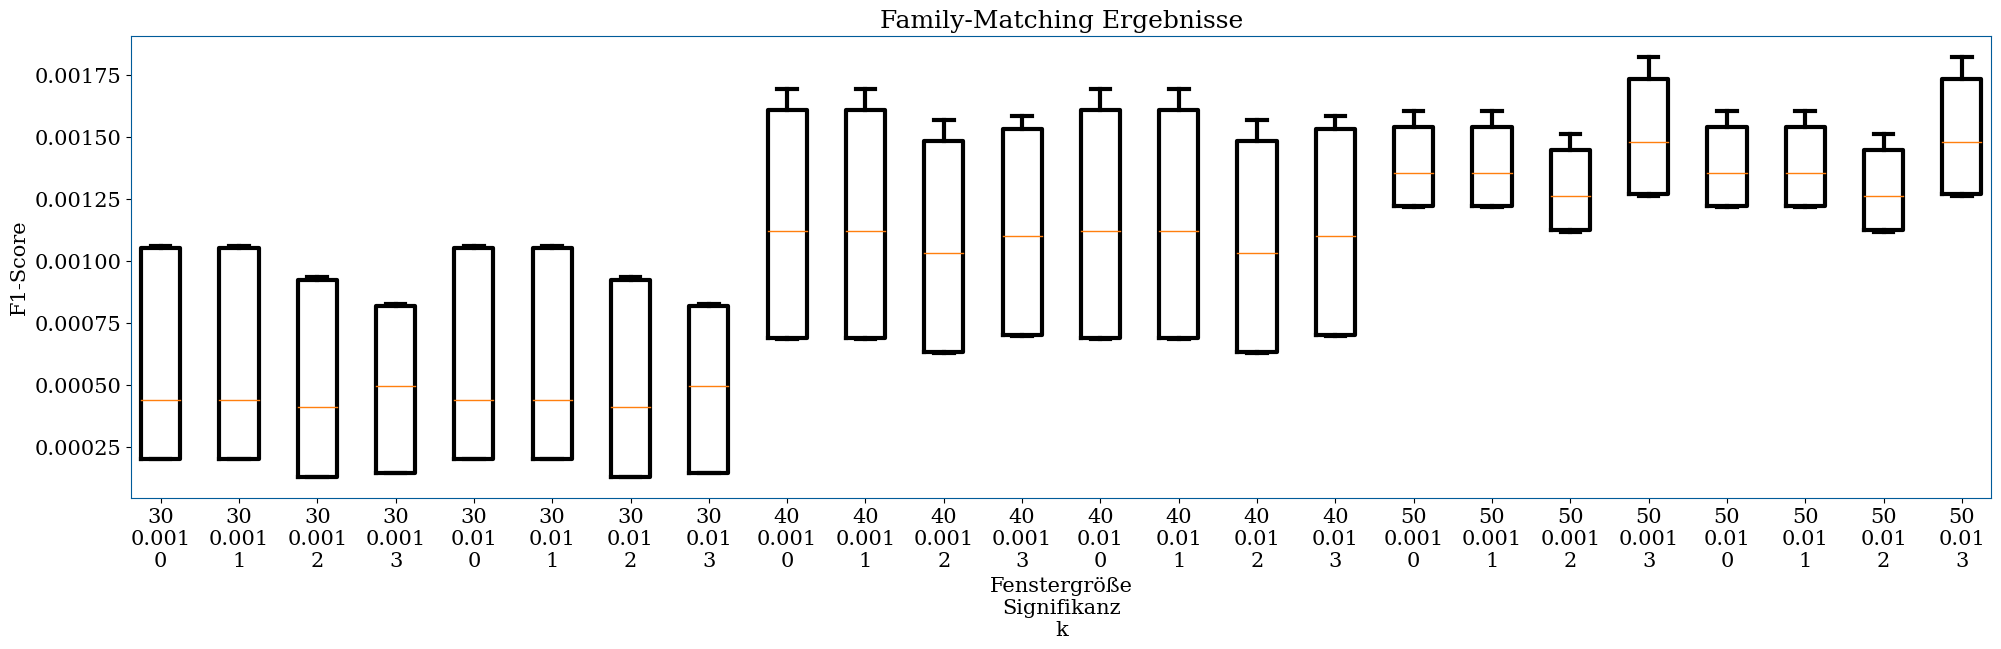
\includegraphics[width=\textwidth]{plot_selection_method.fam.png}
            \caption{bla}
            \label{fig:selection_method.fam}
        \end{figure}
% section ergebnisse (end)
